\documentclass[12pt]{article}
\usepackage{amsmath}
\usepackage{geometry}
\usepackage{graphicx}
\usepackage{hyperref}
\usepackage[latin1]{inputenc}
\usepackage{listings}
\renewcommand{\labelitemi}{$\textendash$}
\geometry{
    a4paper,
    total={170mm,257mm},
    left=15mm,
    right=15mm,
    top=5mm,
    bottom=15mm
}

\title{CS4061: Week 3 Assignment}
\author{Conor McCauley - 17323203}
\date{October 26, 2020}

\begin{document}

\maketitle

\noindent \textbf{Dataset Identifier:} \texttt{\# id:9--18--9}

\section*{Question (i)}

\noindent (a) The below plot shows the values from the dataset. Both input features, $x_1$ and $x_2$, are plotted along the x-axis and y-axis, respectively, while the target value is plotted along the z-axis:

\begin{center}
    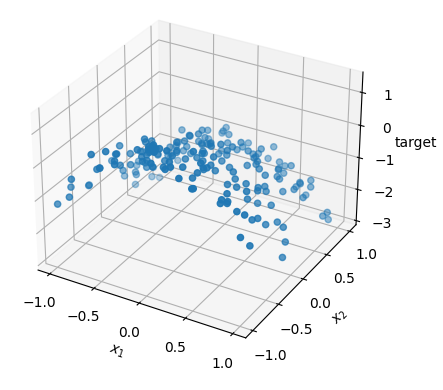
\includegraphics[scale=0.55]{fig_1.png}
\end{center}

The training data appears to be in the form of a curve as opposed to a plane. This can be seen more clearly when you view the plot head-on as follows:

\begin{center}
    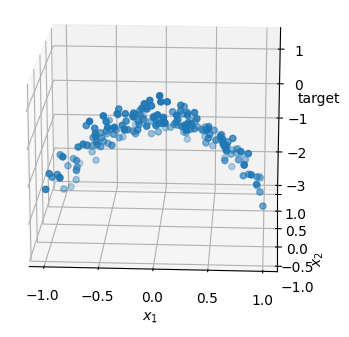
\includegraphics[scale=0.65]{fig_2.png}
\end{center}

\noindent (b) We can add additional polynomial features to our training data using the following code:

\begin{center}
    \lstset{basicstyle=\footnotesize}
    \begin{lstlisting}[language=Python]
    X = np.column_stack((X1, X2))
    X_poly = PolynomialFeatures(5).fit_transform(X)
    \end{lstlisting}
\end{center}

Through testing different values of $C$ I found that $C = 1$ was the minimum value such that all parameter values (except, of course, the intercept) were zero. As such, the values of $C$ that I chose to use were $1$, $10$ and $1000$. It's important to note that the value we pass into SciKit's \texttt{Lasso} function is not $C$ but $\alpha$, which, in this case, is equivalent to $\frac{1}{2C}$. The following code is used to train all of the models:

\begin{center}
    \lstset{basicstyle=\footnotesize}
    \begin{lstlisting}[language=Python]
    C_range = [1, 10, 1000]
    for C in C_range:
        model = Lasso(alpha=1/(2*C)).fit(X_poly, Y)
    \end{lstlisting}
\end{center}

The models trained using these values of $C$ produced the following parameter values:

\begin{center}
    \begin{tabular}{|c|p{0.8\linewidth}|}
        \hline
        $C$ & $\theta$ \\
        \hline
        $1$ & $-0.59, 0, 0, 0, 0, 0, 0, 0, 0, 0, 0, 0, 0, 0, 0, 0, 0, 0, 0, 0, 0, 0$ \\
        \hline
        $10$ & $-0.22, 0, 0, -0.88, -1.31, 0, 0, 0, 0, 0, 0, 0, 0, 0, 0, 0, 0, 0, 0, 0, 0, 0$ \\
        \hline
        $1000$ & $0.07, 0, 0, -0.96, -1.68, 0.06, 0, 0, 0, 0, -0.13, -0.28, 0.23, 0, -0.31, 0,$ $-0.26, 0, 0.75, 0.15, -0.42, 0$ \\
        \hline
    \end{tabular}
\end{center}

Smaller values of $C$ increase the cost penalty at each iteration and, seeing as lasso regression attempts to reduce the effect of less important features on predictions by keeping as many parameter values as close to zero as possible, this increased cost penalty results in many (if not all) of the parameter values being close to or equal to zero for smaller values of $C$. As $C$ is increased and the resulting cost penalty is decreased many of the parameter values begin to diverge further away from zero. This effect can be seen in the above table.

\noindent (c) Given that the dataset contained input features in the range $(-1, 1)$ I chose to predict values in the extended range $(-3, 3)$ at intervals of $0.5$. The test data was generated using Numpy and, as in (b), additional polynomial features were added using SciKit:

\begin{center}
    \lstset{basicstyle=\footnotesize}
    \begin{lstlisting}[language=Python]
    X_test = np.mgrid[-3:3.5:0.5, -3:3.5:0.5].reshape(2, -1).T
    X_test_poly = PolynomialFeatures(5).fit_transform(X_test)
    \end{lstlisting}
\end{center}

Predictions were then made for each of the models from (b) and the resulting values were plotted alongside the training data. The predictions are represented by a blue continuous surface while the training data are represented by red markers. In order to make the visualisation easier to understand I also included a view of each plot from an alternate angle:

\begin{center}
    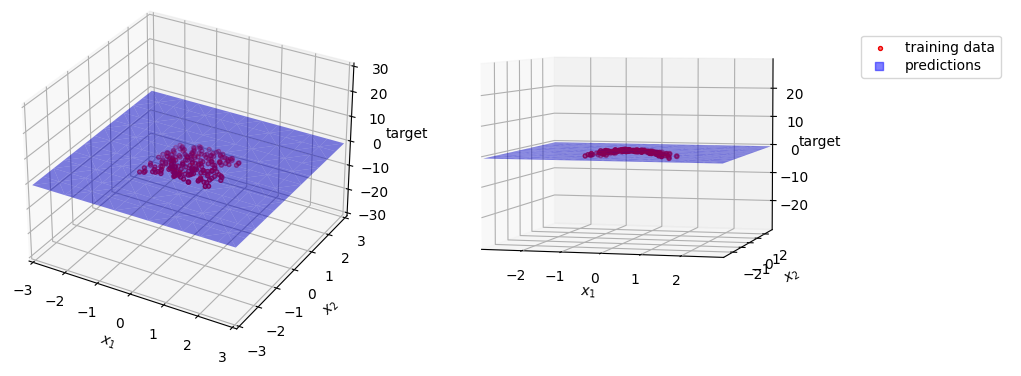
\includegraphics[scale=0.65]{fig_3.png}
    $C = 1$
    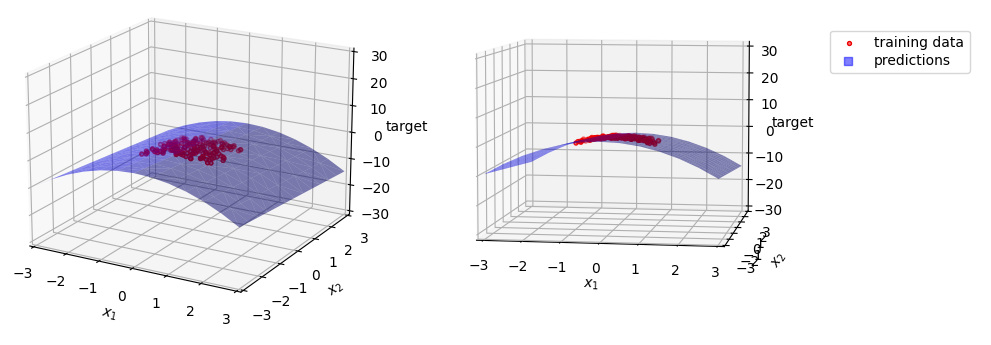
\includegraphics[scale=0.65]{fig_4.png}
    $C = 10$
    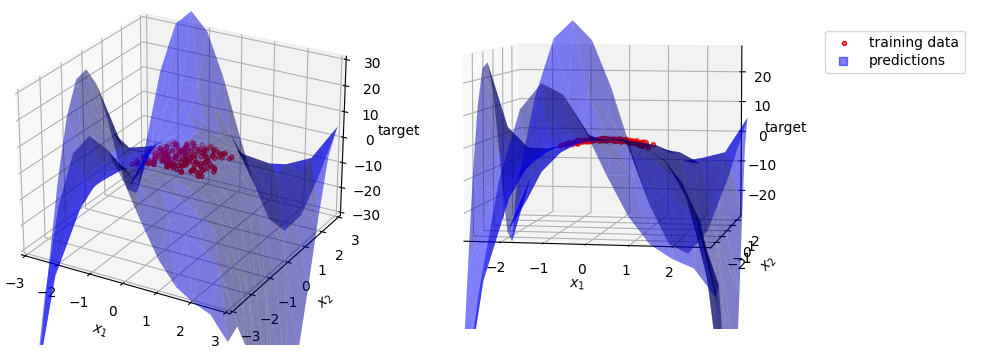
\includegraphics[scale=0.65]{fig_5.png}
    $C = 1000$
\end{center}

When $C = 1$ all of the parameter values (except the intercept) are zero. This leads to a flat plane very roughly aligned with the training data. In this case we can say that our model is under-fitting and wouldn't make correct predictions for the training data, let alone the test data. When $C = 1000$ the model appears to correctly predict target values for the training data but produces somewhat bizarre values for a lot of the test data. This seems to be a clear example of over-fitting and it's likely that noise in the training data played a part in the model producing such strange predictions. When $C = 10$ the predictions seem to make a lot more sense and the resulting surface appears to cleanly continue the curve produced by the training data. As such, $C = 10$ appears to be the optimal choice for this dataset.

\noindent (d) As discussed in (c) under-fitting is when a model fails to model the training data and is also incapable of predicting values for new test data while over-fitting is when a model begins to factor noise and randomness from the training data into its predictive model which also results in it failing to predict values for new test data. Smaller values of $C$ can lead to under-fitting as cost penalties are higher leading to the model keeping many/all parameter values very close to zero which results in a poor predictive model. When $C$ is larger the inverse occurs: high costs are not penalised as much which leads to larger parameter values and a tendency for noise and randomness in the training data to be factored into the predictive model.

\noindent (e) In order to implement a ridge regression model for (b) and (c) only two aspects of the code needed to be changed: the range of $C$ values were altered, and the \texttt{Lasso} function was replaced with the \texttt{Ridge} function. The remaining code was not modified and does not need to be re-explained.

As in (b), through testing different values of $C$ I found that $C = 10^{-4}$ was the minimum value such that all parameter values (except the intercept) were quite close to zero. As such, the values of $C$ that I chose to use were $10^{-4}$, $10^{-3}$ and $10^{-1}$. Once again, it's important to note that the value we pass into SciKit's \texttt{Ridge} function is not $C$ but $\alpha$, which is equivalent to $\frac{1}{2C}$. The following parameter values were produced:

\begin{center}
    \begin{tabular}{|c|p{0.8\linewidth}|}
        \hline
        $C$ & $\theta$ \\
        \hline
        $10^{-4}$ & $-0.59, 0, 0, -0.01, -0.01, 0, 0, 0$ $, 0, 0, -0.01, 0, 0, 0, 0, 0, 0, 0, 0, 0, 0, -0.01$ \\
        \hline
        $10^{-2}$ & $-0.56, 0, 0, -0.11, -0.06, 0, 0, 0, -0.03, -0.01, -0.07, -0.05, 0, -0.02, -0.01, 0,$ $0, -0.02, 0, -0.02, -0.01, -0.05$ \\
        \hline
        $10^{-1}$ & $-0.20, 0, -0.04, -0.77, -0.96, 0.03, 0.05, -0.01, -0.06, 0.02, -0.26, -0.70, 0.08,$ $-0.25, -0.11, -0.01, -0.01, 0, 0.10, 0.04, 0, -0.09$ \\
        \hline
    \end{tabular}
\end{center}

\textbf{N.B.} while many of the values in the above table are zero this is solely due to my limiting each value to two decimal places - in actuality, while many of the values are very small, none of them are equal to zero.

As was the case in (b), smaller values of $C$ lead to more features being kept close to zero (although never equal to zero) while larger values of $C$ lead to more divergent parameter values. A key difference between the values produced via ridge regression and lasso regression is that in ridge regression none of the features are eliminated entirely, i.e. equal to zero, so we fail to entirely remove features with poorer predictive performance.

We will use the same extended range of $(-3, 3)$ to predict values using our models. The result plots are as follows:

\begin{center}
    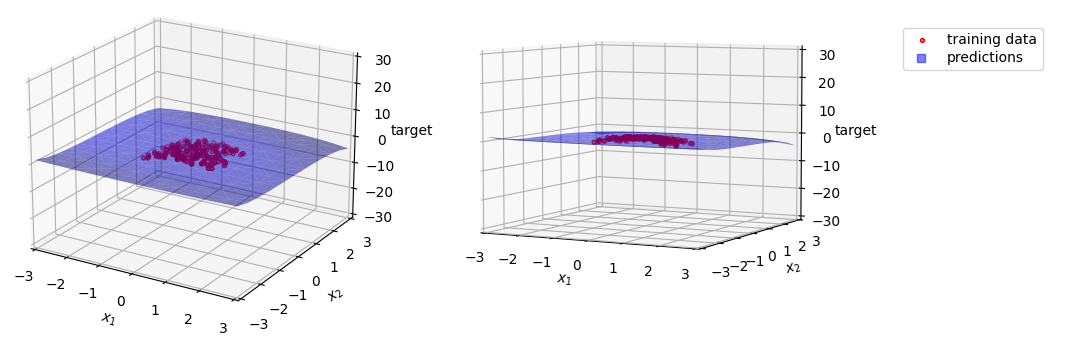
\includegraphics[scale=0.65]{fig_6.png}
    $C = 10^{-4}$
    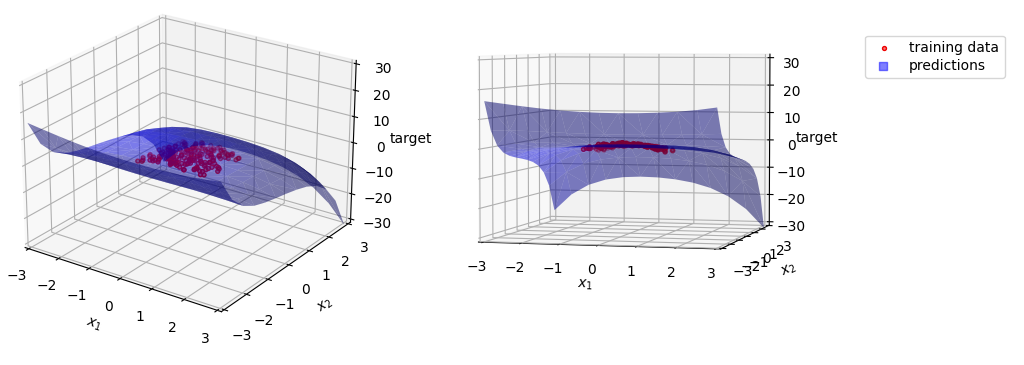
\includegraphics[scale=0.65]{fig_7.png}
    $C = 10^{-3}$
    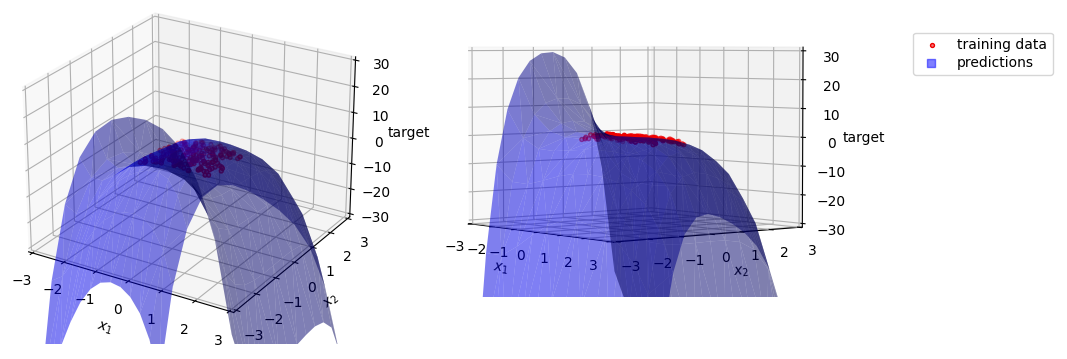
\includegraphics[scale=0.65]{fig_8.png}
    $C = 10^{-1}$
\end{center}

For $C = 10^{-4}$ we end up with an \textit{almost} entirely flat and under-fitting plane as was the case with $C = 1$ for lasso regression. The slight curves at the edges of our test range are due to ridge regression not entirely removing any of the features from the model. For $C = 10^{-3}$ and $C = 10^{-1}$ both models seem to correctly predict values for the training data while appearing to over-fit slightly as evidenced by the curves on either end of the test range (this is especially pronounced for $C = 10^{-1}$. This apparent over-fitting, again, may be caused by ridge regression not entirely eliminating any of the poorer features from the predictions.

It would appear that lasso regression with $C = 10$ is the optimal choice here as it fit the model better than other values of $C$ we chose for lasso regression. As mentioned in (a), given the apparent simplicity of the curve produced by our training data, lasso regression is the superior choice over ridge regression as our simple training data can be modelled sparsely using few coefficients - something ridge regression does not really support.

\section*{Question (ii)}

\noindent (a) We can train a lasso regression model with $C = 1$ as in (i) and use SciKit's \texttt{cross\_val\_score()} method to run cross-validation on our model for a number of different values of $k$:

\begin{center}
    \lstset{basicstyle=\footnotesize}
    \begin{lstlisting}[language=Python]
    model = Lasso(alpha=1/(2*C)).fit(X_poly, Y)
    k_range = [2, 5, 10, 25, 50, 100]
    for k in k_range:
        scores = cross_val_score(model, X_poly, Y, cv=k, scoring='neg_mean_squared_error')
    \end{lstlisting}
\end{center}

We can also use SciKit's \texttt{DummyRegressor} to generate a dummy model as a baseline predictor for each value of $k$:

\begin{center}
    \lstset{basicstyle=\footnotesize}
    \begin{lstlisting}[language=Python]
    dummy = DummyRegressor(strategy='mean').fit(X_poly, Y)
    k_range = [2, 5, 10, 25, 50, 100]
    for k in k_range:
        dummy_scores = cross_val_score(dummy, X_poly, Y, cv=k,
                        scoring='neg_mean_squared_error')
    \end{lstlisting}
\end{center}

We can then plot the mean and standard deviation (SD) of the mean square error for each of the values of $k$ (I also plotted the mean and variance just to be safe) - this plot also continues the mean square error of the baseline model which, incidentally, reports the exact same values as the trained model (which is why the yellow bar isn't visible):

\begin{center}
    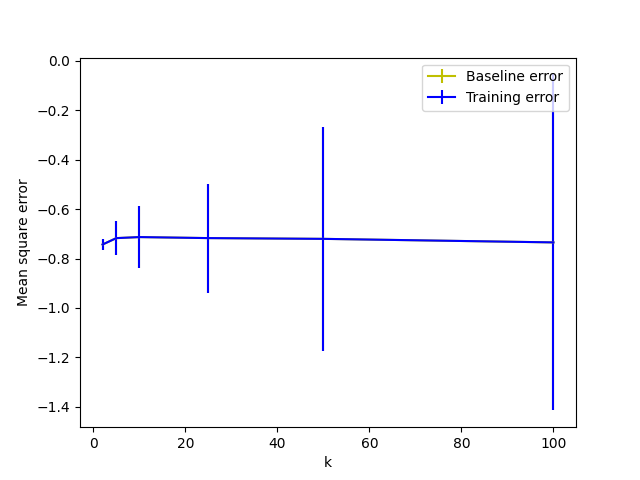
\includegraphics[scale=0.65]{fig_9.png}
    
    Mean and SD against $k$
    
    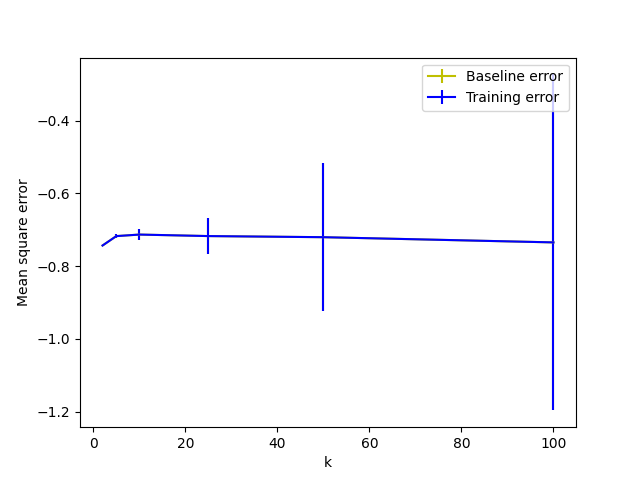
\includegraphics[scale=0.65]{fig_10.png}
    
    Mean and variance against $k$
\end{center}

The exact mean, standard deviation and variance values that were produced are as follows:

\begin{center}
    \begin{tabular}{|c|c|c|c|}
        \hline
        $k$ & Mean & SD & Variance \\
        \hline
        $2$ & $-0.743$ & $0.022$ & $0.000$ \\
        \hline
        $5$ & $-0.717$ & $0.068$ & $0.005$ \\
        \hline
        $10$ & $-0.713$ & $0.124$ & $0.015$ \\
        \hline
        $25$ & $-0.717$ & $0.221$ & $0.048$ \\
        \hline
        $50$ & $-0.720$ & $0.452$ & $0.204$ \\
        \hline
        $100$ & $-0.735$ & $0.680$ & $0.462$ \\
        \hline
    \end{tabular}
\end{center}

When choosing a suitable value for $k$ an important factor is the size of the dataset. If both $k$ and our dataset are large then we will need to train many models each containing a large number of data points - this greatly increases the computation time. However, in this case, given the relatively small size of our dataset this is not really a problem for us. Conversely, if $k$ is too small then our models will be trained on an inadequate number of data points leading to inaccurate parameter values and poor predictions. Due to this effect and given the size of our dataset we don't want to choose a value of $k$ that is too small.

Taking into account the above plot and the aforementioned trade-offs it would seem that $k = 2$ is a deal more inaccurate than all of the rest while values of $k \geq 25$ have standard deviations that are much too large to produce consistently accurate results. The optimal choice seems to be between $k = 5$ and $k = 10$. While $k = 10$ does have a slightly better mean error its standard deviation is almost twice as large as $k = 5$ which will lead to less consistent results - for this reason it would appear that $k = 5$ is the optimal choice for our dataset.

\noindent (b) As mentioned in (a), I chose 5-fold cross-validation and plotted the mean and SD of the mean square error for the following values of $C \in \{0.1, 1, 10, 100, 1000\}$. These values of $C$ were chosen as, using our visualisations from (i), we could see that this broad range contains examples of both under-fitting and over-fitting which would imply that the ideal value of $C$ would lie somewhere within this range - I chose to increase each successive value of $C$ by a factor of $10$ as this is the standard choice as mentioned in lectures.

As in (a), SciKit's \texttt{DummyRegressor} was used to fit a baseline model. The following plot, which uses a logarithmic x-axis for ease of visualisation, displays the mean and SD of the mean square error for both the lasso model and the baseline model:

\begin{center}
    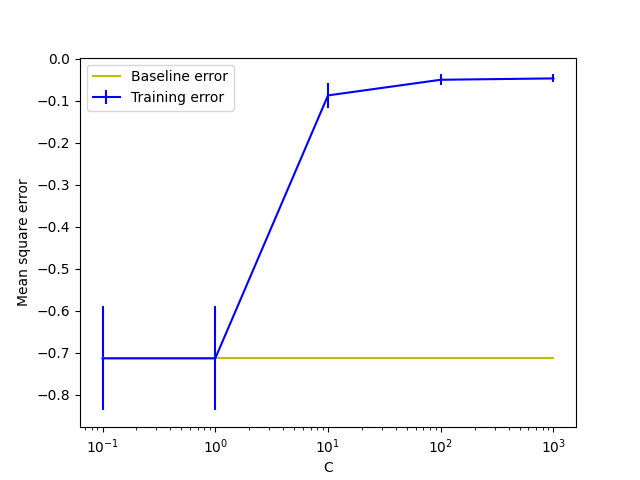
\includegraphics[scale=0.65]{fig_11.png}
\end{center}

\noindent (c) Based solely on the results from (b) it would appear that $C = 100$ or $C = 1000$ are among the optimal choices for $C$. However, if we take into account our visualisations and discussions from (i) it would seem that $C = 1000$ is over-fitting the dataset and could lead to poor predictions on new, unseen data. We can also dismiss values of $C \leq 1$ as they don't even outperform the baseline and led to under-fitting in (i). It appears that the appropriate choices are $C = 10$ and $C = 100$, and, given the slightly better mean square error and smaller SD of $C = 100$, I believe it's the optimal choice.

\noindent (d) I, again, chose 5-fold cross-validation and plotted the mean and SD of the mean square error for the following values of $C \in \{10^{-5}, 10^{-4}, 10^{-3}, 10^{-2}, 10^{-1}\}$. My reasoning for choosing these values of $C$ was essentially the same as the reasoning given for lasso regression in (b): both under-fitting and over-fitting were seen in the visualisation from (i) implying the ideal value lies somewhere in between. A baseline predictor was created in the same way as before and the following plot was produced:

\begin{center}
    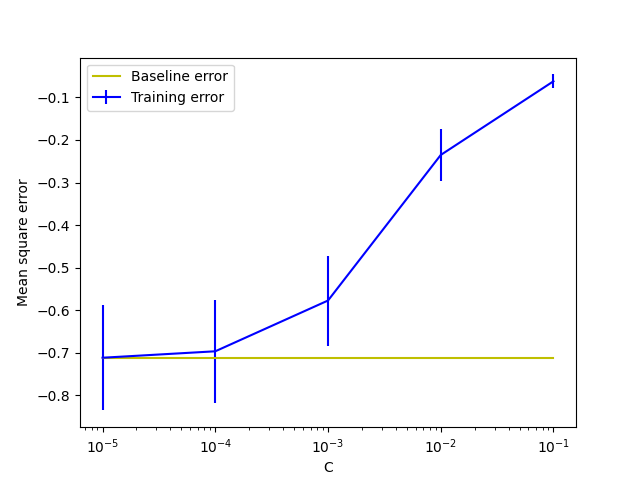
\includegraphics[scale=0.65]{fig_12.png}
\end{center}

Based on this result we should be able to dismiss values of $C \leq 10^{-4}$ as they barely outperform the baseline predictor and our model for $C = 10^{-4}$ was clearly under-fitting the dataset in (i). While $C = 10^{-1}$ has a low mean square error in this model, it seemed to be over-fitting the dataset in (i). As such, out of the two remaining options, $C = 10^{-3}$ and $C = 10^{-2}$, it seems that the much better mean square error and smaller SD of $C = 10^{-2}$ leads to it definitely being the optimal choice.

\section*{Appendix: Code}

\lstset{basicstyle=\footnotesize}
\begin{lstlisting}[language=Python]
from matplotlib import cm
from mpl_toolkits.mplot3d import Axes3D
from sklearn.dummy import DummyRegressor
from sklearn.linear_model import Lasso, Ridge
from sklearn.metrics import accuracy_score
from sklearn.model_selection import cross_val_score
from sklearn.preprocessing import PolynomialFeatures
import matplotlib.pyplot as plt
import numpy as np
import pandas as pd

# select specific feature from the data
def filter_data(data, index):
    return [d[index] for d in data]

# plot the training data as well as a model's predicted results
def plot_training_data_and_predictions(training_data, pred_data, pred_results):
    fig = plt.figure()
    ax = fig.add_subplot(111, projection='3d')
    # plot predictions
    X1 = filter_data(pred_data, 0)
    X2 = filter_data(pred_data, 1)
    ax.plot_trisurf(X1, X2, pred_results, vmin=-100, vmax=100, color='#0000ff80')
    # plot training data
    X = filter_data(training_data, 0)
    Y = filter_data(training_data, 1)
    Z = filter_data(training_data, 2)
    ax.scatter(X, Y, Z, c='#ee000088', edgecolors='#ee0000', s=8)
    # configure and show plot
    ax.zaxis.set_rotate_label(False)
    ax.set_xlabel('$x_1$')
    ax.set_ylabel('$x_2$')
    ax.set_zlabel('target', rotation=0)
    ax.set_xlim3d(-3, 3)
    ax.set_ylim3d(-3, 3)
    ax.set_zlim3d(-30, 30)
    plt.show()

def part_i_a(data):
    X = filter_data(data, 0)
    Y = filter_data(data, 1)
    Z = filter_data(data, 2)
    fig = plt.figure()
    ax = fig.add_subplot(111, projection='3d')
    ax.scatter(X, Y, Z)
    ax.set_xlabel('$x_1$')
    ax.set_ylabel('$x_2$')
    ax.zaxis.set_rotate_label(False)
    ax.set_zlabel('target', rotation=0)
    plt.show()

def part_i_bc(data, is_lasso=True):
    # generate new polynomial features
    X1 = np.array(filter_data(data, 0)).reshape(-1, 1)
    X2 = np.array(filter_data(data, 1)).reshape(-1, 1)
    X = np.column_stack((X1, X2))
    X_poly = PolynomialFeatures(5).fit_transform(X)
    Y = np.array(filter_data(data, 2))
    # generate grid of feature values using Numpy magic
    X_test = np.mgrid[-3:3.5:0.5, -3:3.5:0.5].reshape(2, -1).T
    X_test_poly = PolynomialFeatures(5).fit_transform(X_test)
    # train models and make predictions
    C_range = [1, 10, 1000] if is_lasso else [0.0001, 0.001, 0.1]
    for C in C_range:
        if is_lasso: model = Lasso(alpha=1/(2*C)).fit(X_poly, Y)
        else: model = Ridge(alpha=1/(2*C)).fit(X_poly, Y)
        predictions = model.predict(X_test_poly)
        print(f'C = {C} >> intercept = {model.intercept_}, coefs = {list(model.coef_)}')
        plot_training_data_and_predictions(data, list(X_test), list(predictions))

def part_i(data):
    part_i_a(data)
    part_i_bc(data, is_lasso=True)
    part_i_bc(data, is_lasso=False)

def part_ii_a(data):
    # generate new polynomial features
    X1 = np.array(filter_data(data, 0)).reshape(-1, 1)
    X2 = np.array(filter_data(data, 1)).reshape(-1, 1)
    X = np.column_stack((X1, X2))
    X_poly = PolynomialFeatures(5).fit_transform(X)
    Y = np.array(filter_data(data, 2))
    # train models and run cross-validations
    C = 1
    k_range = [2, 5, 10, 25, 50, 100]
    model = Lasso(alpha=1/(2*C)).fit(X_poly, Y)
    dummy = DummyRegressor(strategy='mean').fit(X_poly, Y)
    means, stds, _vars = [], [], []
    dummy_means, dummy_stds, dummy_vars = [], [], []
    for k in k_range:
        # calculate baseline scores
        dummy_scores = cross_val_score(dummy, X_poly, Y, cv=k,
                        scoring='neg_mean_squared_error')
        dummy_means.append(dummy_scores.mean())
        dummy_stds.append(dummy_scores.std())
        dummy_vars.append(pow(dummy_scores.std(), 2))
        # calculate model scores
        scores = cross_val_score(model, X_poly, Y, cv=k, scoring='neg_mean_squared_error')
        mean, std, var = scores.mean(), scores.std(), pow(scores.std(), 2)
        means.append(mean)
        stds.append(std)
        _vars.append(var)
        print(f'k = {k} >> mean = {mean}, std = {std}, var = {var}')
    # plot mean and SD for each k
    plt.errorbar(k_range, dummy_means, yerr=dummy_stds, fmt='y')
    plt.errorbar(k_range, means, yerr=stds, fmt='b')
    plt.xlabel('k')
    plt.ylabel('Mean square error')
    plt.legend(['Baseline error', 'Training error'])
    plt.show()
    # plot mean and variance for each k
    plt.errorbar(k_range, dummy_means, yerr=dummy_vars, fmt='y')
    plt.errorbar(k_range, means, yerr=_vars, fmt='b')
    plt.xlabel('k')
    plt.ylabel('Mean square error')
    plt.legend(['Baseline error', 'Training error'])
    plt.show()

def part_ii_b(data, is_lasso=True):
    # generate new polynomial features
    X1 = np.array(filter_data(data, 0)).reshape(-1, 1)
    X2 = np.array(filter_data(data, 1)).reshape(-1, 1)
    X = np.column_stack((X1, X2))
    X_poly = PolynomialFeatures(5).fit_transform(X)
    Y = np.array(filter_data(data, 2))
    # initialse k and C
    k = 10
    if is_lasso: C_range = [0.1, 1, 10, 100, 1000]
    else: C_range = [0.00001, 0.0001, 0.001, 0.01, 0.1]
    # calculate baseline scores
    dummy = DummyRegressor(strategy='mean').fit(X_poly, Y)
    dummy_scores = cross_val_score(dummy, X_poly, Y, cv=k,
                    scoring='neg_mean_squared_error')
    dummy_mean = dummy_scores.mean()
    # train models and run cross-validations
    means, stds = [], []
    for C in C_range:
        if is_lasso: model = Lasso(alpha=1/(2*C)).fit(X_poly, Y)
        else: model = Ridge(alpha=1/(2*C)).fit(X_poly, Y)
        scores = cross_val_score(model, X_poly, Y, cv=k, scoring='neg_mean_squared_error')
        mean, std, var = scores.mean(), scores.std(), pow(scores.std(), 2)
        means.append(mean)
        stds.append(std)
        print(f'C = {C} >> mean = {mean}, std = {std}, var = {var}')
    # plot mean and std for each C
    plt.errorbar(C_range, [dummy_mean] * len(C_range), fmt='y')
    plt.errorbar(C_range, means, yerr=stds, fmt='b')
    plt.xlabel('C')
    plt.ylabel('Mean square error')
    plt.xscale('log')
    plt.legend(['Baseline error', 'Training error'])
    plt.show()
        
def part_ii(data):
    part_ii_a(data)
    part_ii_b(data, is_lasso=True)
    part_ii_b(data, is_lasso=False)

data = pd.read_csv('dataset.csv', comment='#').values.tolist()
part_i(data)
part_ii(data)
\end{lstlisting}

\end{document}
